\documentclass[dvipsnames, tikz]{standalone}
\usepackage{amsmath}
\usepackage{arevmath}
\usepackage{xcolor}
\usepackage{tikz}
\usetikzlibrary{calc}
\usetikzlibrary{decorations.pathreplacing,calligraphy,3d}
\usetikzlibrary{matrix,shapes,fit,backgrounds}

\begin{document}
	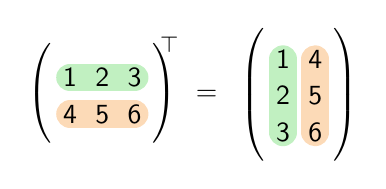
\begin{tikzpicture}[
		%Global config
		>=latex,
		line width=1pt,
		color = black,
		every left delimiter/.style={xshift=1ex},
		every right delimiter/.style={xshift=-1ex},
		%Styles
		Matrix/.style={
			matrix of nodes,
			%text height=2.5ex,
			%text depth=0.75ex,
			%text width=3.25ex,
			%align=center,
			left delimiter=(,
			right delimiter=),
			%column sep=1pt,
			%row sep=1pt,
			%nodes={draw=black!10}, % Uncoment to see the square nodes.
			%nodes in empty cells,
		},
		DA/.style={
			fill,
			opacity=0.2,
			rounded corners,
			inner sep=-3pt,
			line width=1pt,
		},
		DG/.style={
			line cap = round,
			rounded corners=0.25ex,
			line width = 10pt,
			opacity = 0.3,
		}
		]
		
		\matrix[Matrix] at (0,0) (M){ % Matrix contents  
			\sf 1 & \sf 2 & \sf 3 \\
			\sf 4 & \sf 5 & \sf 6 \\
		};
		\draw (0.85,0.65) node {\footnotesize $\top$};
		\draw (1.075+0.25,0) node {=};
		\matrix[Matrix] at (2.5,0) (M2){ % Matrix contents  
			\sf 1 & \sf 4 \\
			\sf 2 & \sf 5 \\
			\sf 3 & \sf 6 \\
		};
	
		\begin{scope}[on background layer] 
			%To delimit internal area groups
			%\node[DA,blue,fit=(M-3-2)(M-5-4)](subM-2){};
			%\node[DA,green,fit=(M-6-4)(M-7-6)](subM-3){};
			
			% For line sectors
			\draw[DG,LimeGreen](M-1-1.center) --(M-1-3.center); 
			\draw[DG,LimeGreen](M2-1-1.center) --(M2-3-1.center); 
			\draw[DG,BurntOrange](M-2-1.center) --(M-2-3.center); 
			\draw[DG,BurntOrange](M2-1-2.center) --(M2-3-2.center); 
			%\draw[DG,LimeGreen](M3-1-1.center) --(M3-1-1.center); 
			%\draw[DG,NavyBlue](M-1-2.center) --(M-3-4.center);
			%\draw[DG,PineGreen](M-1-3.center) --(M-2-4.center);
			%\draw[DG,BrickRed](M-2-1.center) --(M-3-2.center);
			%\draw[DG,BurntOrange](M-3-1.center) --(M-3-1.center);
			%\draw[DG,LimeGreen](M-1-4.center) --(M-1-4.center);
		\end{scope}
		
	\end{tikzpicture}
\end{document}